\section{Control}

Being able to establish the dynamics equations of a robot is still not enough to make it carry out a desired trajectory. There are several disturbances in physical systems that cannot be modelled, which means that a controlling scheme is required to alleviate the influence of those disturbances. The following schematic gives an overview of a typical control architecture:

\begin{center}
	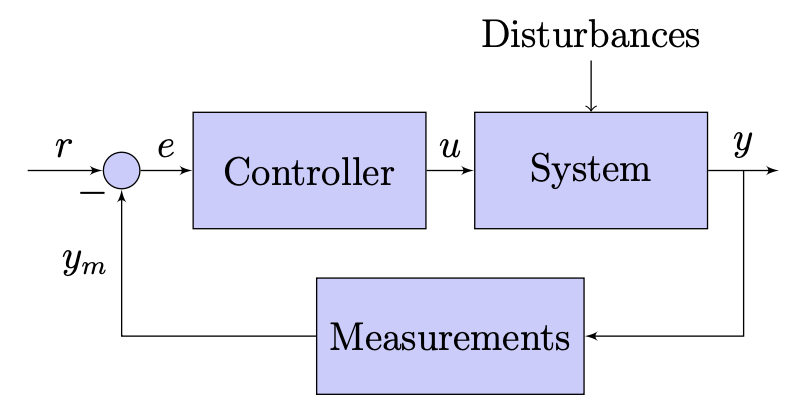
\includegraphics[width=8cm]{sections/imgs/7_control_architecture.png}
\end{center}

The value $r$ would be the desired state of the system. Computing the difference $e=y_{m}-r$ yields the error of the current state $y_{m}$ with respect to the desired state. The controller takes $e$ into account when generating control signals $u$, in order to correct any error introduced by disturbances.

This section is based on the explanations in exercise 5, \href{https://www.youtube.com/watch?v=5-k2RzfIgoU&list=PL65CC0384A1798ADF&index=14}{lecture 13} and \href{https://www.youtube.com/watch?v=U3diaQ-iU0I&list=PL65CC0384A1798ADF&index=16}{lecture 14}.

\subsection{Mass-Spring-Systems}

As a prerequisite to understanding the function of a PD controller, mass-spring-systems have been studied in the lecture. The importance of these systems lies in their connection to the behaviour of the error $e$ in control problems. We will later see that the error $e$ behaves like a mass-spring-system itself.

\begin{center}
	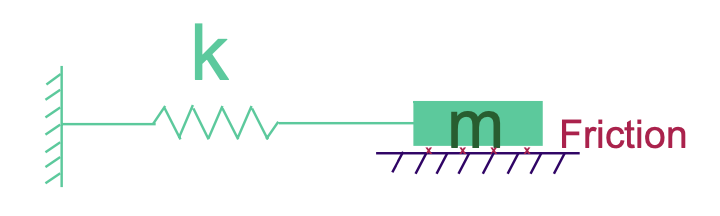
\includegraphics[width=4cm]{sections/imgs/7_mass_spring_system.png}
\end{center}

The dynamic equation of the mass-spring-system is:

\begin{center}
	$m \ddot{x}+b \dot{x}+k x=f$
\end{center}

where $m$ is the mass of the object, $b$ is the friction constant and $k$ is the spring constant. The deflection of the object from its resting position is  denoted by $x$. This equation is, in the context of control, also called the \textit{open-loop-equation}, since it does not take into account any feedback from the system (like, e.g., in the case of a robot, joint position measurements from sensors or such).

We distinguish three possible cases for the applied force $f$: Under-damping leads to oscillation of the system (spring stiffness dominates), while over-damping leads to slow convergence to the resting position (friction dominates). Critical damping leads to the fastest possible transition of the system to its resting configuration, avoiding both overdamping and underdamping (friction and stiffness are in balance).

\begin{center}
	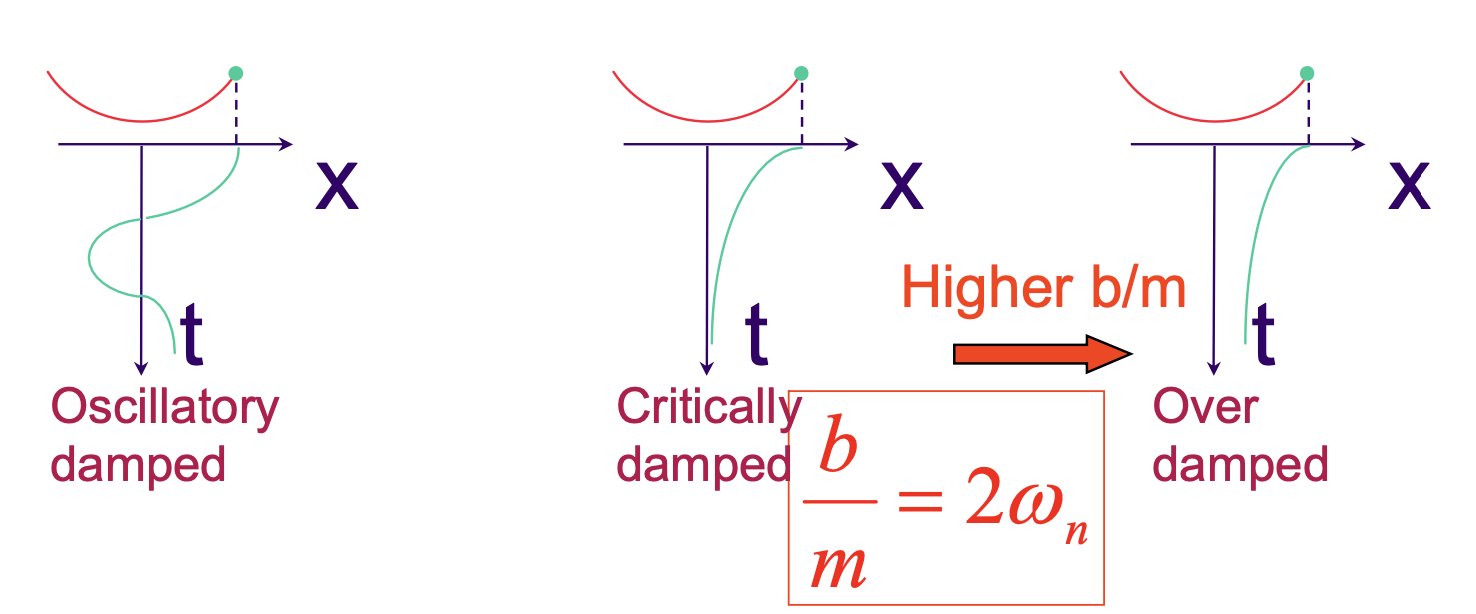
\includegraphics[width=7cm]{sections/imgs/7_critically_damped.png}
\end{center}

\subsubsection{Solution of the Dynamic Equation (Position Control)}

How can we achieve critical damping? The force $f$ that we exert on the object must depend on friction and spring forces, and we can assume that it’s of the form $f=-k_{p} x-k_{v} \dot{x}$ (proportional-derivative-/ PD-control; the formula is derived \href{https://youtu.be/5-k2RzfIgoU?t=3514}{here in the lecture}). This yields the \textit{closed-loop equation}:

\begin{center}
	$m \ddot{x}+\left(b+k_{v}\right) \dot{x}+\left(k+k_{p}\right) x=0$
\end{center}

We are interested in controlling the movement of the body, so we are interested in determining the function $x(t)$, which means we need to solve the differential equation. This is done by solving the characteristic equation:

\begin{center}
$m s^{2}+\left(b+k_{v}\right) s+\left(k+k_{p}\right)=0$	
\end{center}

The solutions to this quadratic equation are given by the well-known formula
$$
s_{1,2}=\frac{-\left(b+k_{v}\right) \pm \sqrt{\left(b+k_{v}\right)^{2}-4 m\left(k+k_{p}\right)}}{2 m}=\frac{-b^{\prime} \pm \sqrt{b^{\prime 2}-4 m k^{\prime}}}{2 m} .
$$
It is then common to abbreviate $\left(b+k_{v}\right)$ as $b^{\prime}$ and $\left(k+k_{p}\right)$ as $k^{\prime}$. The solutions $s_{1}, s_{2}$ determine the trajectory $x(t)$ as follows:
$$
x(t)=c_{1} e^{s_{1} t}+c_{2} e^{s_{2} t}
$$

A special case is $s_{1}=s_{2} \in \mathbb{R}$. This case corresponds to critical damping of the system. Note that this can be achieved by choosing $b^{\prime}$ and $k^{\prime}$ such that $b^{\prime 2}-4 m k^{\prime}=0$, or $b^{\prime}=2 \sqrt{m k^{\prime}}$ (we can assume $b^{\prime}$ and $k^{\prime}$ to be positive). In the case of an oscillating system, the equations can also be stated in a different form:

\begin{center}
$s^{2}+2 \zeta \omega_{n} s+\omega_{n}^{2}=0$
\end{center}

with the ``damping ratio'' $\zeta$ and the ``natural frequency'' $\omega_{n}$
 
\begin{center}
$
\begin{aligned}
\zeta &=\frac{b^{\prime}}{2 \sqrt{k^{\prime} m}} \\
\omega_{n} &=\sqrt{\frac{k^{\prime}}{m}}.
\end{aligned}
$
\end{center}

Now, we design our PD-controller by setting $k_p$ and $k_v$, such that we achieve critical damping (see the experiments in \href{https://www.youtube.com/watch?v=U3diaQ-iU0I&list=PL65CC0384A1798ADF&index=16}{lecture 14} for an example). Herein, if the damping ratio $\zeta$ is too small, the joint oscillates and if it is too large, it is overdamped (reaches the goal state slower). Moreover, the natural frequency $\omega$ is limited by an upper bound, as explained in the next section. If this upper bound is exceeded, the motion becomes unstable.
\subsubsection{Resonance}

Until now, we assumed that all parts of the mechanic systems we observed do not deform at all. But in reality, components of robots have a finite stiffness, which means that they deform minimally under stress. This can lead to the undesired effect of resonance, which leads to deformations adding up until finally components may be damaged.

A simple possibility of taking the effect of resonance into account is through enforcing the following inequality:
$$
\omega_{n} \leq \frac{1}{2} \omega_{\text {res }}
$$
Here, $\omega_{\text {res }}$ is the so-called resonant frequency of the object. If this condition holds, we can be sure that no undesired resonances occur.

\subsubsection{Control Partitioning}

Until now, we have used the following simple rule to influence the behaviour of a mass-spring system:
$$
f=-k_{p} x-k_{v} \dot{x}
$$
Using this rule, we were able to achieve critical damping of a mass-spring system, choosing parameters $k^{\prime}$ and $b^{\prime}$ according to $b^{\prime}=2 \sqrt{m k^{\prime}}$. However, the choice of $b^{\prime}$ depends on $m$, which is acceptable for a simple mass-spring system, but makes things very complicated in more complex systems. Thus, we want to decouple the mass-dependent part from the equation, using an extended rule that reads as follows:
$$
f=\alpha f^{\prime}+\beta
$$
This equation is known as the \textit{model-based portion}. Through this rule, we want to achieve the following: Factors $\alpha$ and $\beta$ should be chosen such that the system, considering only $f^{\prime}$ as input, behaves like a unit mass, governed by the equation
$$
\ddot{x}=f^{\prime}
$$
Writing down the complete equation for the system, we obtain
$$
m \ddot{x}+b \dot{x}+k x=\alpha f^{\prime}+\beta .
$$

Now comes the interesting part: How should we choose $\alpha$ and $\beta$ in order to achieve the desired effect? Obviously, $\beta=b \dot{x}+k x$ and $\alpha=m$ must hold. Note that we are now able to influence the system directly through $f^{\prime}$. This is the decoupled open-loop equation. Again, be aware that for the simple case of a mass-spring system there is not much gained through rewriting the system like this, but for manipulating more complicated systems, the advantage is substantial.

Now, we move again from the open-loop form to the closed-loop form. Thus, let $f^{\prime}$ again depend on spring force and friction force, such that
$$
f^{\prime}=-k'_{p} x-k'_{v} \dot{x}
$$
with some new constants $k_{p}'$ and $k_{v}'$. The equation of motion becomes
$$
\ddot{x}+k'_{p} x+k'_{v} \dot{x}=0
$$
In particular, we see that now $k_{v}$ and $k_{p}$ are now independent of system parameters. The system will always be critically damped if $k_{v}'=2 \sqrt{k'_{p}}$.

In other words, we want to approximate the mass-spring system with a unit mass system that is linearly scaled by $\alpha$ and $\beta$. Herein, $\alpha$ compensates for the mass ($m$ or the mass matrix $M$) and $\beta$ compensates for $b\dot x+kx$ (or other terms like centrifugal, coreolis and gravitational forces with $V$ and $G$). All terms that depend on $m$ cancel out and we are left with the equation for the unit mass system, for which we then design $k'_{v}$ and $k'_{p}$ independent of the mass.
\\

\begin{minipage}[c]{0.45\textwidth}
	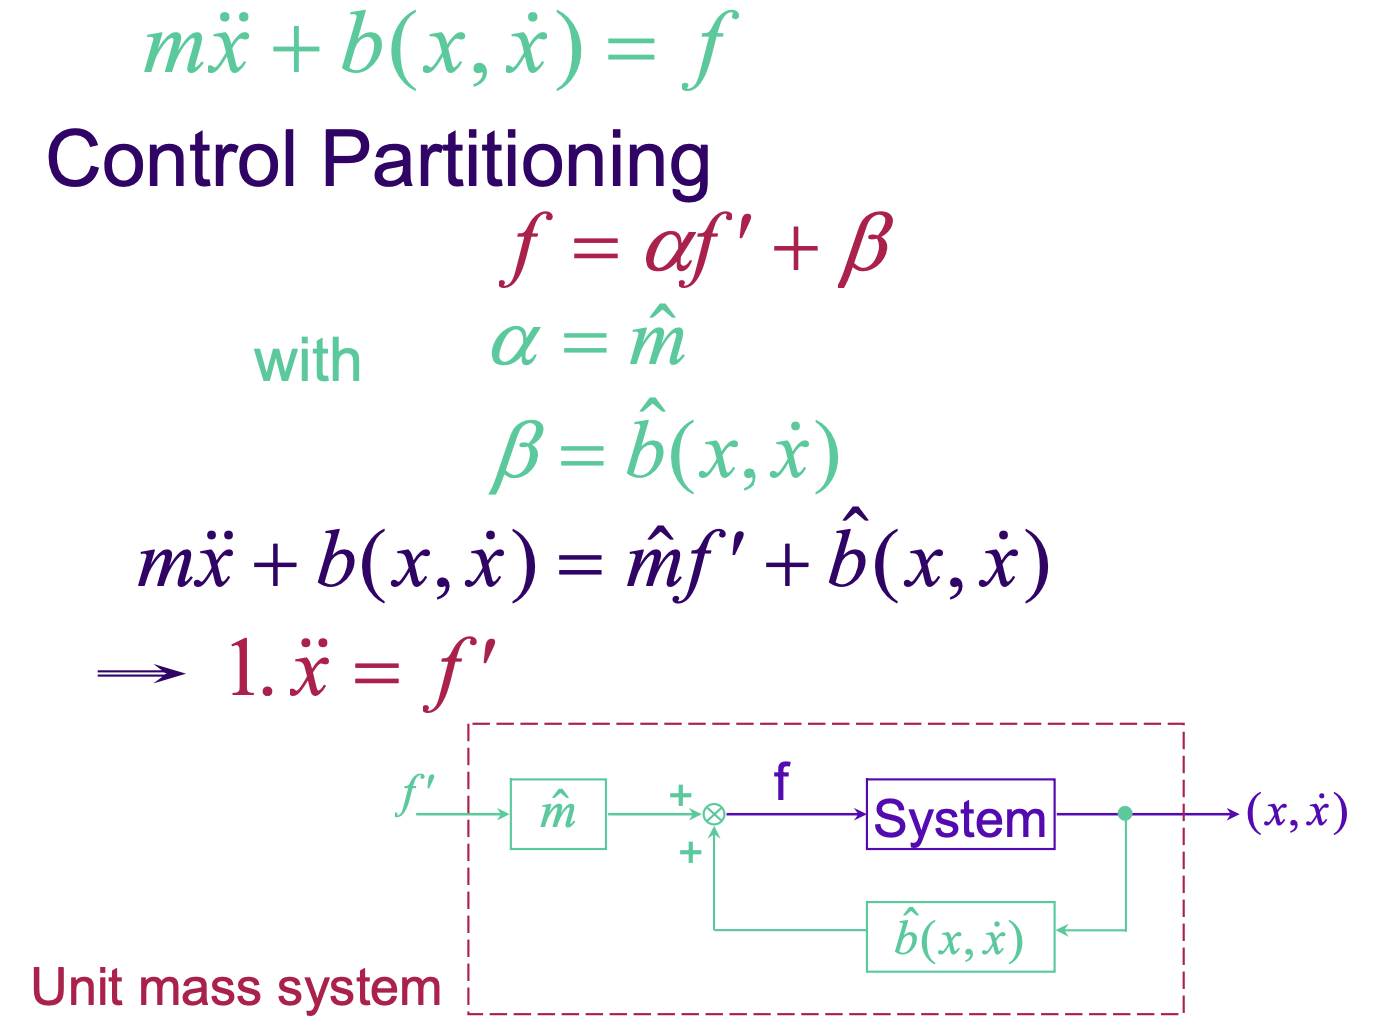
\includegraphics[width=7cm]{sections/imgs/7_control_partitioning.png}
\end{minipage}
\hfill
\begin{minipage}[c]{0.45\textwidth}
In the slide on the left, the non-linear system $m\ddot x+b(x,\dot x)=f$ is approximated (through control partitioning) with the factors $\alpha$ and $\beta$. This equation is equivalent to $f'=\ddot x$ (the other terms cancel out), which is the unit mass system. The control loop shows how the unit mass system is linearly scaled with the factor $\hat m$ and $\hat b(x, \dot x)$.
\end{minipage}

\subsubsection{Trajectory following/ Motion Control}

Now we no longer assume that we are simply interested in achieving critical damping of a mass-spring system, but instead we want the system to carry out a certain trajectory. The computed trajectory shall be denoted by $x_{d}(t)$, and we assume that $x_{d}(t)$ is a twice continuously differentiable function. Let $e(t)=x_{d}(t)-x(t)$ denote the difference between the actual position and the desired position.
Movement along the desired trajectory can now be achieved by employing the following control rule (\textit{servo-portion} for trajectory following/ ``servo control law''):
$$
f^{\prime}=\ddot{x}_{d}+k_{v} \dot{e}+k_{p} e
$$
Substituting this rule into the partition scheme, we obtain:
$$
\ddot{x}=\ddot{x}_{d}+k_{v} \dot{e}+k_{p} e \Leftrightarrow \ddot{e}+k_{v} \dot{e}+k_{p} e=0
$$
We see that the error $e$ now behaves like a mass-spring system! This means that we can achieve critical damping of the error through appropriate choice of $k_{p}$ and $k_{v}$. This means that the error will tend towards 0 , and it will approach 0 with a speed depending on $k_{v}$ and $k_{p}$ - critical damping will thus provide the fastest possible convergence of the error towards 0. 
\\

\begin{minipage}[c]{0.45\textwidth}
	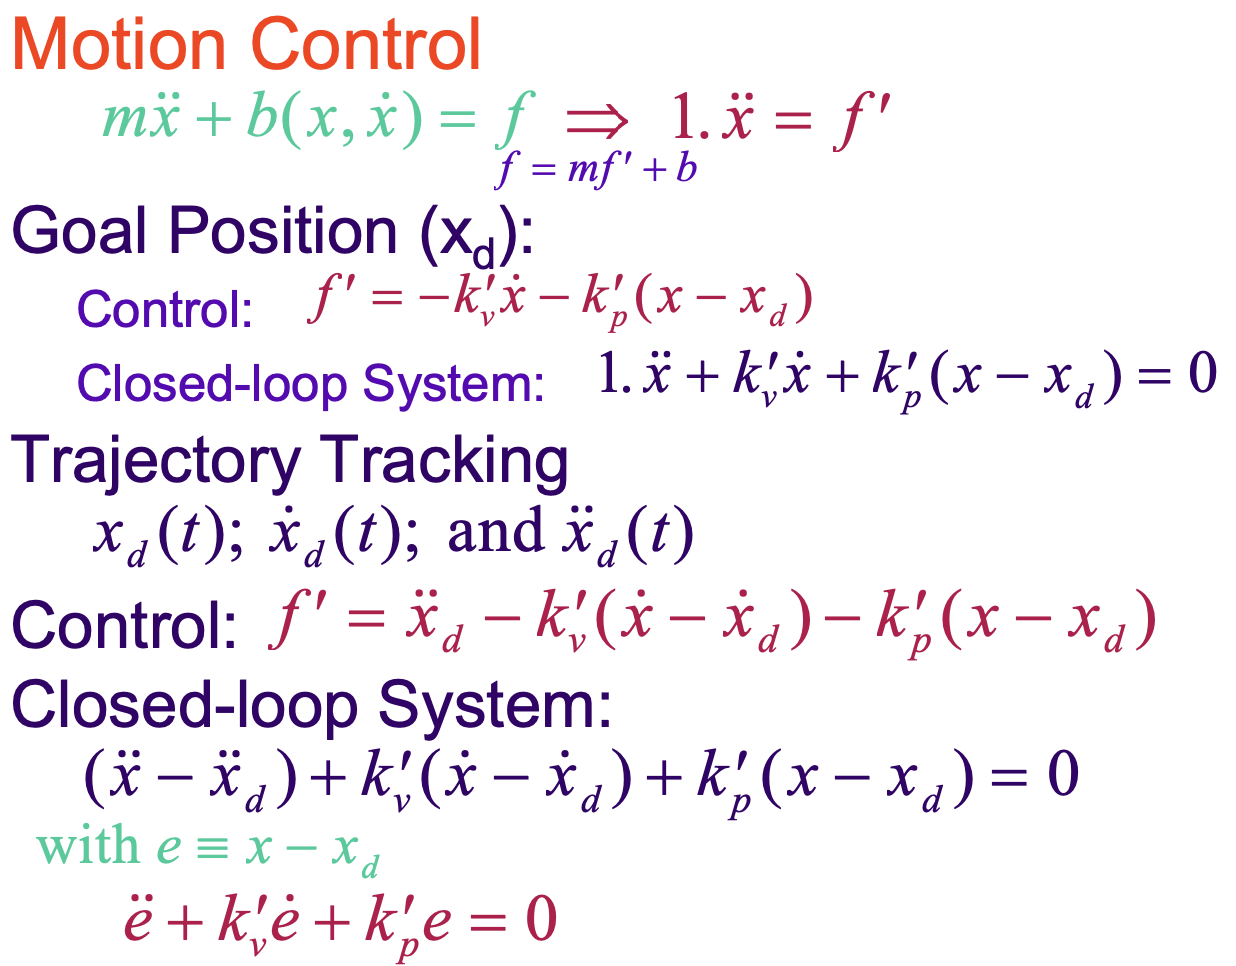
\includegraphics[width=7cm]{sections/imgs/7_motion_control.png}
\end{minipage}
\hfill
\begin{minipage}[c]{0.45\textwidth}
The slide on the left summarises the control rules used for position control and trajectory tracking (controlling the error). The respective control force then leads to the closed-loop equation.
\end{minipage}


Note that this is only true if there are no further unmodeled effects present in the system - in practice, one usually employs a PID controller (PD controller with additional integral part) to assure that the error always approaches $0 .$
What we have discussed here is a mathematical treatment of the PD-controller. Above derivation explains the typical oscillating behaviour of PD-controllers. Furthermore, we see that it is possible to compute the proportional and differential factors directly.

\subsubsection{Multi-dimensional systems}

The decoupling method might not seem very useful at first sight, because it does not really help much with the simple case of a mass-spring-system with only one object. The main advantage of using this partitioning scheme is that it greatly simplifies the control problem for multi-dimensional problems. Assuming that $x$ is a multi-dimensional quantity, the equations of motion without partitioning will look like this:
$$
M \ddot{x}+B \dot{x}+K x=f
$$
Here we can as well adopt the approach of using system feedback, in hope of achieving critical damping for that system. We set the controlling force
$$
f=-K_{v} \dot{x}-K_{p} x
$$
with some matrices $K_{v}$ and $K_{p}$, and we end up with:
$$
M \ddot{x}+\left(B+K_{v}\right) \dot{x}+\left(K+K_{p}\right) x=0
$$
This is a multi-dimensional linear differential equation, and it is quite difficult to handle and to analyze. Determining $K_{v}$ and $K_{p}$ in order to achieve critical damping becomes a \textbf{major} problem when using this approach!

Now let's find out how this works when the partitioning scheme is in use. We set $f=\alpha f^{\prime}+\beta$, where $\alpha=M$, and $\beta=B \dot{x}+K x$. We end up with:
$$
M \ddot{x}+B \dot{x}+K x=M f^{\prime}+B \dot{x}+K x
$$
Assuming that $M$ is invertible, this transforms into
$$
\ddot{x}=f^{\prime}
$$
just as it did in the one-dimensional case. Further setting $f^{\prime}=-K_{v} \dot{x}-K_{p} x$, we end up with the following system:
$$
\ddot{x}+K_{v} \dot{x}+K_{p} x=0
$$

Choosing $K_{p}$ and $K_{v}$ as diagonal matrices with entries $k_{p i}, k_{v_{i}}$, this becomes a series of decoupled differential equations:
$$
\begin{gathered}
\left(\begin{array}{c}
\ddot{x}_{1} \\
\ddot{x}_{2} \\
\vdots \\
\ddot{x}_{n}
\end{array}\right)+\left(\begin{array}{cccc}
k_{v_{1}} & 0 & \ldots & 0 \\
0 & k_{v_{2}} & \ddots & \vdots \\
\vdots & \ddots & \ddots & 0 \\
0 & \ldots & 0 & k_{v_{n}}
\end{array}\right)\left(\begin{array}{c}
\dot{x}_{1} \\
\dot{x}_{2} \\
\vdots \\
\dot{x}_{n}
\end{array}\right)+\left(\begin{array}{cccc}
k_{p_{1}} & 0 & \ldots & 0 \\
0 & k_{p_{2}} & \ddots & \vdots \\
\vdots & \ddots & \ddots & 0 \\
0 & \ldots & 0 & k_{p_{n}}
\end{array}\right)\left(\begin{array}{c}
x_{1} \\
x_{2} \\
\vdots \\
x_{n}
\end{array}\right)=\left(\begin{array}{c}
0 \\
0 \\
\vdots \\
0
\end{array}\right) \Leftrightarrow \\
\left(\begin{array}{c}
\ddot{x}_{1} \\
\ddot{x}_{2} \\
\vdots \\
\ddot{x}_{n}
\end{array}\right)+\left(\begin{array}{c}
k_{v_{1}} \dot{x}_{1} \\
k_{v_{2}} \dot{x}_{2} \\
\vdots \\
k_{v_{n}} \dot{x}_{n}
\end{array}\right)+\left(\begin{array}{c}
k_{p_{1}} x_{1} \\
k_{p_{2}} x_{2} \\
\vdots \\
k_{p_{n}} x_{n}
\end{array}\right)=\left(\begin{array}{c}
0 \\
0 \\
\vdots \\
0
\end{array}\right)
\end{gathered}
$$
Achieving critical damping of this system is extremely easy: Set $k_{v i}=2 \sqrt{k_{p i}}$, and we're done!

\subsection{Manipulator Control}

By using either the Newton-Euler or the Lagrange method, we are already able to determine equations of motion of a robot. The equations, formulated in state-space form, generally look like this:
$$
\tau=M(\Theta) \ddot{\Theta}+V(\Theta, \dot{\Theta})+G(\Theta)
$$
This is a multi-dimensional system, but it's not even linear. It turns out that dealing with a nonlinear system is no problem at all when applying the partitioning scheme. Partitioning works exactly like before (let $\alpha=M(\Theta), \beta=$``everything else'') and leads to an easily controllable system. Applying the well-known partitioning scheme
$$
\tau=\alpha \tau^{\prime}+\beta
$$
with $\alpha=M(\Theta), \beta=V(\Theta, \dot{\Theta})+G(\Theta)$ to our system, we can use the servo control law
$$
\tau^{\prime}=\ddot{\Theta}_{d}+K_{v}\left(\dot{\Theta}_{d}-\dot{\Theta}\right)+K_{p}\left(\Theta_{d}-\Theta\right)
$$
to control our robot. Here, $\Theta_{d}$ is the vector of desired joint positions. The expression $\left(\Theta_{d}-\Theta\right)$ will now be abbreviated as $E$. Inserting above values into the state space equation, we obtain:
$$
\begin{aligned}
M(\Theta) \ddot{\Theta}+V(\Theta, \dot{\Theta})+G(\Theta) &=M(\Theta)\left(\ddot{\Theta}_{d}+K_{v} \dot{E}+K_{p} E\right)+V(\Theta, \dot{\Theta})+G(\Theta) \\
0 &=M(\Theta)\left(\ddot{\Theta}_{d}-\ddot{\Theta}+K_{v} \dot{E}+K_{p} E\right) \\
0 &=\ddot{E}+K_{v} \dot{E}+K_{p} E
\end{aligned}
$$
This is the so-called error equation. Again, we choose $K_{v}$ and $K_{p}$ to be diagonal:
$$
K_{v}=\left(\begin{array}{ccccc}
k_{v 1} & 0 & 0 & \cdots & 0 \\
0 & k_{v 2} & 0 & \cdots & 0 \\
0 & 0 & \ddots & \ddots & \vdots \\
\vdots & \vdots & \ddots & \ddots & 0 \\
0 & 0 & \cdots & 0 & k_{v n}
\end{array}\right), \quad K_{p}=\left(\begin{array}{ccccc}
k_{p 1} & 0 & 0 & \cdots & 0 \\
0 & k_{p 2} & 0 & \cdots & 0 \\
0 & 0 & \ddots & \ddots & \vdots \\
\vdots & \vdots & \ddots & \ddots & 0 \\
0 & 0 & \cdots & 0 & k_{p n}
\end{array}\right)
$$

As before, we end up with a couple of independent error equations, and each one of those can be seen as a mass-spring model that we whish to damp critically. The equations would be
$$
\ddot{e}_{i}+k_{v_{i}} \dot{e}_{i}+k_{p_{i}} e_{i}=0 .
$$
When talking about natural frequencies in the context of manipulator control, we are referring to the natural frequency associated with those error equations. This means that the following simple relationship holds:
$$
\omega_{n i}=\sqrt{k_{p i}} .
$$
Finally, critical damping can be achieved as usual by letting
$$
k_{v i}=2 \sqrt{k_{p i}}
$$